\documentclass{sig-alternate}
\usepackage[utf8]{inputenc}
\usepackage[T1]{fontenc}

\newcommand{\superscript}[1]{\ensuremath{^{\textrm{#1}}}}
\def\sharedaffiliation{\end{tabular}\newline\begin{tabular}{c}}
\def\wu{\superscript{*}}
\def\wg{\superscript{\dag}}

\usepackage{listings} 

% Typography
\usepackage{times}
\usepackage{mathptmx}
\usepackage{microtype}
\usepackage[normalem]{ulem}
\usepackage[pdftex,bookmarks,bookmarksopen,bookmarksdepth=2,
            urlcolor=black,colorlinks=true,linkcolor=black,citecolor=black]{hyperref}
\usepackage[capitalize,noabbrev]{cleveref}
\def\UrlFont{\em}

% Graphics
\usepackage{tikz}
\usepackage{tkz-graph}
\usetikzlibrary{arrows,positioning,shapes.misc}
\usepackage{graphicx}
\definecolor{lightgrey}{RGB}{170, 170, 170}
\definecolor{darkblue}{RGB}{0, 0, 0}
\definecolor{darkred}{RGB}{170, 0, 0}
\definecolor{darkgreen}{RGB}{0, 110, 0}

% Acronyms
\usepackage{xspace}
\newcommand{\sparql}{{SPARQL}\xspace}
\newcommand{\sparqlo}{{SPARQL 1.1}\xspace}
\newcommand{\arq}{{ARQ}\xspace}
\newcommand{\wthreec}{{W\oldstylenums 3C}\xspace}
\newcommand{\sfive}{{S\oldstylenums 5}\xspace}
\newcommand{\select}{{SELECT}\xspace}
\newcommand{\construct}{{CONSTRUCT}\xspace}
\newcommand{\ask}{{ASK}\xspace}
\newcommand{\describe}{{DESCRIBE}\xspace}
\newcommand{\from}{{FROM}\xspace}
\newcommand{\odbc}{{odbc}\xspace}

% Tight lists
\usepackage{enumitem}
\setlist{nolistsep}

% Listings and Verbatim environment
\usepackage{fancyvrb}
\usepackage{relsize}
\usepackage{listings}
\usepackage{verbatim}
\newcommand{\smalllistingsize}{\fontsize{8pt}{9.5pt}}
\newcommand{\inlinelistingsize}{\fontsize{8.5pt}{11pt}}
\newcommand{\defaultlistingsize}{\inlinelistingsize}
\RecustomVerbatimCommand{\Verb}{Verb}{fontsize=\inlinelistingsize}
\RecustomVerbatimEnvironment{Verbatim}{Verbatim}{fontsize=\inlinelistingsize}
\lstset{frame=lines,captionpos=b,numberbychapter=false,escapechar=§,
        belowskip=1em,
        xleftmargin=2ex,
        framexleftmargin=2ex,
        basicstyle=\ttfamily\smalllistingsize\selectfont}
\crefname{lstlisting}{Listing}{Listings}
\definecolor{grey}{RGB}{130,130,130}

\usepackage{color}
\newcommand{\todo}[1]{\noindent\textcolor{red}{{\bf \{TODO}: #1{\bf \}}}}
\newdef{definition}{Definition}

\begin{document}

\title{Studying public transit API query logs\\ to get an indication of travel flows}
\numberofauthors{6}
\author{
\alignauthor
Pieter Colpaert\\
\affaddr{\email{\texttt{pieter.colpaert@ugent.be}}}
\and
\alignauthor
Alvin Chua\\
\affaddr{\email{\texttt{alvin.chua@asro.kuleuven.be}}}
\and
\alignauthor
Ruben Verborgh\\
\affaddr{\email{\texttt{ruben.verborgh@ugent.be}}}
\and
\alignauthor
Erik Mannens\\
\affaddr{\email{\texttt{erik.mannens@ugent.be}}}
\and
\alignauthor
Rik Van de Walle\\
\affaddr{\email{\texttt{rik.vandewalle@ugent.be}}}
\and
\alignauthor
Andrew Vande Moere\\
\affaddr{\email{\texttt{andrew.vandemoere\\@asro.kuleuven.be}}}\\
}

\maketitle
\begin{abstract}

%Public transit schedules are made available on the Web in various ways, such as in a GTFS file, a route planning API, or through Linked Connections.
%This webservice provides an answer to a route planning question with parameters such as ``departuretime'', ``from'' and ``to''.
% Context & % Need
In the field of urban planning, researchers need an indication of how people move between cities. 
Yet, getting statistics of travel flows within public transit systems has proven to be troublesome.
% Task
We analyzed the query logs of the iRail API, a high expressive route planning API for the Belgian railways, to get an indication of travel flows between cities in Belgium.
We were able to study $\sim$100k to 500k requests for each month between October 2012 and November 2015, which is between $0.5\%$ and $1.7\%$ of the amount of monthly passengers.
% Object & Findings
Using data visualizations, we illustrated the commuting patterns in Belgium and show that Brussels, the capital, acts as a central hub. The Flemish region appears to be polycentric, while in the Walloon region, everything converges on Brussels.
The findings correspond to the real travel demand, say experts of the passenger federation Trein Tram Bus.
% Conclusion
We conclude that query logs of route planners are of high importance in getting an indication of the travel flows.
% Perspectives
High expressive transport data publishing methods such as route planning API exist, as well as low expressive data dumps or data fragments.
In order to be able to gather meaningful logs in all cases, we suggest using a separate POST request containing the entire query.

\end{abstract}

\vspace{1em}

\section{Introduction}
\label{sec:introduction}

\todo{Rework introduction at the end}

%Today, public transport data still remains absent from the Linked Open Data cloud\footnote{\url{http://lod-cloud.net/}}.
%Bizarre, one could notice, as many open transport datasets are already available, according to the Global Open Data Index of 2014\footnote{\url{http://index.okfn.org/dataset/timetables/2014/}}.
%We can imagine that, what contributed to this, are the de-facto standard ways to publish public transit data to the Web.
%There are currently two ways, as illustrated in \cref{fig:LDFAxis1}: publishing data using the General Transit Feed Specification (GTFS) and offering a route planning service.

%\emph{GTFS}, on the one hand, is a data dump format: it is a compressed ZIP-file, containing a couple of CSV-files, describing the rules for when a public transit vehicle will pass by on a certain location.
%The specification is a huge success: up to date, it is supported among all current open source route planning software systems, and it is used in products such as \emph{CityMapper}, \emph{Ally}, \emph{Navitia.io}, \emph{Google Maps} and \emph{Bing Maps}.
%Persistence of the identifiers used within these datasets, is not a requirement, neither is it an ambition of the format\footnote{\url{https://groups.google.com/forum/#!msg/gtfs-changes/Z8Mf31MaZms/8Hc9F4psAQAJ}}.
%The goal of GTFS is to create an exchange format which specific software packages can use to transform it into their format of choice.

%On the other hand, public transit agencies also publish their data by providing \emph{route planners}.
%These route planner offer a query service on top of the data and expose these over the Web.
%However, when machines should access these, rate limiters are common place: only a limited amount of queries should be done in order for the service to be able to stay online.

%
% Linked Data Fragments axis
\begin{figure}[t]
  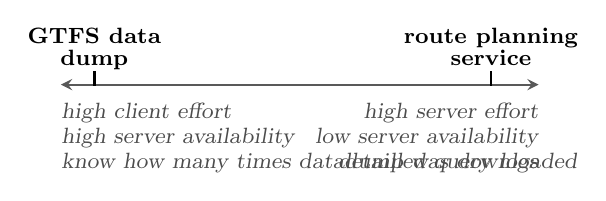
\begin{tikzpicture}[
    x=.005\textwidth,
    y=.1cm,
    axis/.style={
      line width=.8pt,
      stealth-stealth,
      color=black!65,
    },
    axislabel/.style={
      inner sep=0,
      font=\slshape\fontsize{8}{9}\selectfont,
      color=black!70,
    },
    tick/.style={
      line width=1pt,
    },
    ticklabel/.style={
      anchor=south,
      inner sep=0,
      align=center,
      font=\bfseries\fontsize{8}{8}\selectfont,
      text depth=0pt,
    },
  ]
    \newcommand\tick[2]{%
      \draw[tick] (#1, 1.7) -- (#1, -.4pt);
      \node[ticklabel] at (#1, 2.4) {#2};
    }
    \newcommand\vaguetick[1]{%
      \draw[tick,densely dotted] (#1, 1.7) -- (#1, -.4pt);
    }

    \draw[axis] (-100, 0) -- (0, 0);
    \node[axislabel,align=left,anchor=north west] at (-100, -2.3)
    {
%      generic requests\\
      high client effort\\
      high server availability\\
      know how many times datadump was downloaded
    };
    \node[axislabel,align=right,anchor=north east] at (0, -2.3)
    {
%      specific requests\\
      high server effort\\
      low server availability\\
      detailled query logs
    };

    \tick{-93}{GTFS data\\dump}
    \tick{-10}{route planning\\service}
%    \tick{-32}{Linked\\Connections}

   % \vaguetick{-84}
   % \vaguetick{-52}
   % \vaguetick{  5}
   % \vaguetick{-10}
   % \vaguetick{ 28}
   % \vaguetick{ 55}

   %\node[align=center,font=\fontsize{8}{9}\selectfont\bfseries] at (0, -8.3)
   %   {various types of\\Linked Data Fragments};
  \end{tikzpicture}
  \caption{
    This axis illustrates two extremes. With GTFS data dumps, the data reusers do all the work, and no query logs can be gathered. With route planning services, the servers need to do all the work, yet detailled query logs can be studied.
  }
  \label{fig:LDFAxis1}
\end{figure}

Getting indications of people flows through public transit networks is a challenge.
The data is tedious to get, mainly with public transit systems where passengers don't have to check-in and check-out.
Nevertheless, people are calculating their intended routes by using the Web.
\emph{Can we get an indication of these transit flows by studying the query logs of Web-services?}

The \emph{iRail} project\footnote{\url{http://hello.irail.be}} started in 2008 to make the data of the Belgian railway accessible for developers.
Ever since, the project offers developer both a GTFS data dump for third party apps and a route planning API.
The query logs of this API has been stored since 2013.
We study these query logs by creating a couple of visualizations which illustrate a couple of patterns.
Two of the documented patterns in this paper correspond to reality, another does not.

In this paper, we give a small overview of related work to gather data for flow analysis.
Next, we study the iRail query logs to find out whether we can find interesting patterns.
Finally, we look at Linked~Connections~\cite{lc}, a proposed new way of publishing queryable public transit data, and whether we would still be able to have an indication of the transit flows with a Linked Data Fragments~\cite{ldf} approach.

\section{Related work}
\label{sec:relwork}

\todo{Write relwork at the end}

\emph{Flow analysis} is a topic of theoretical interest and practical importance in various disciplines. 
Flow analysis is conventionally conducted to study spatial dynamics and identify routine patterns in the movement of people.
For instance, interest in modelling traffic flows emerged from the strain placed on urban transportation systems during peak hours~\cite{roth,ferreira}.
Likewise, insight into routine travel patterns is crucial for the conceptualisation of functional urban areas~\cite{servillo,sykora}, urban hierarchies~\cite{christaller} and other territorial structures.

Over the past decade, large datasets have become increasingly commonplace due to the proliferation of sensor networks and portable devices like smartphones.
Termed ``Big Data'' due to the large volume of data records that emerge from real-time sensing\cite{kitchin}, such datasets typically contain information of activities or processes linked to the space and time where they occur.
In the domain of ``Smart City'' research, much has been accomplished with the use of ``Big Data'' to monitor human movement.
Smart card data from public transport systems~\cite{roth,beecham}, taxi journeys~\cite{ferreira} as well as cellular call data~\cite{sevtsuk} have provided planners with new opportunities to develop greater understanding of mobility patterns in urban environments~\cite{batty}.

Visualisation is frequently used to make data analysis tangible, so that the results can be communicated and debated \todo{Robinson, 2008 -121}. This is crucial for our research since the questions presented are exploratory in nature \todo{Kraak, 2008 -150} and can be addressed in many ways. Movement data has received substantial attention from the visualisation community and a range of techniques has been developed to support analysis \todo{Andrienko, 2012 -196}. Of these techniques, flow visualisations facilitate the comparison of aggregated movement over space and time. There are three types of flow visualisations: Line based representations preserves the complete trajectory while matrix type representations take only the start and end locations into account.

Line based representations indicate movement on a path with the shape of the line. The thickness of each line is scaled to the volume of flow along a path. The direction of flow is commonly indicated with an arrowhead. This representation is detailed and straightforward to understand but becomes cluttered when lines intersect. A number of solutions have been proposed for clutter reduction. Filtering is the most commonly practiced. The same goal can be achieved by clustering lines that have similar properties like common start, end or intermediate locations \todo{Andrienko, 2007 -198}. Hierarchical \todo{Guo, 2009 -199} and density based \todo{Rinzivillo, 2008 -201} clustering have also been introduced for this purpose. Both solutions are effective at reducing clutter yet it should be noted that excessive aggregation or filtering removes a significant amount of information from the visualisation. Another solution to reduce clutter is to transform the visual representation. This is achieved by rerouting \todo{Phan, 2005 -88} or bundling \todo{Hurter, 2014 -200} lines in close proximity so that they appear grouped. Unlike clustering, this solution changes the shape of lines by way of interpolation to obtain an ideal layout. In most cases, the interpolation is regulated by conditions to avoid intersections and follow key geographic features such as roads, rivers or coastlines so that the layout appears natural. This solution emphasises major flows within the visualisation since large groups gain visual dominance. Nonetheless, there are two drawbacks to this solution. First, short distance flows that may be important at local scales are de-emphasised or lost in the transformation. Next, the lines do not depict actual paths of movement thus this solution may not be suitable for applications that require strict geographic accuracy.

Matrix type representations are frequently used when the origin and destination preside over intermediate locations on the path of movement. This type of representation is referred to as origin-destination (OD) matrix. Rows and columns correspond to locations while cells are coloured to express the volume of flow. OD matrices can be reordered to emphasise connectivity between locations but the lack of geographic context is a distinct disadvantage. Several solutions have been developed to address this shortcoming. These are based on the notion of small multiples: The matrix is arranged in a geographical order so that the cells correspond to locations on the map. Then, a smaller map of the geographical context is nested in each cell to enable more intuitive comparisons \todo{Guo, 2006 -202}. The limitation of this solution is similar to other forms or small multiples in general - the layout space allocated to each nested map becomes smaller as the number of cells increase. In this instance, nesting detailed geographical maps is problematic since majority of the geographical features become illegible due to scaling. OD Map \todo{Wood, 2010 -86} proposes to nests a series of geographically ordered matrices that are more expressive of spatial relations and remain legible even when a small amount of layout space allocated to each cell.

\section{The query logs}
\label{sec:logs}

The iRail API is a XML/JSON HTTP API where each request on \url{http://api.irail.be} returns a response that can be used directly in an end-user app. It contains four features: 
\begin{enumerate}
\item \emph{Route Planning} (\url{http://api.irail.be/connections/{?from,to,date,time}}) plans a route from one station to another, taking into account a preferred start time.
\item \emph{Next Departures} (\url{http://api.irail.be/liveboard/{?station,date,time}}) shows the next train departures in a certain station, useful for creating quick overviews.
\item \emph{Trip Status} (\url{http://api.irail.be/vehicle/{?id,date}}) returns the stations this train passes by on the day of the request.
\item \emph{List of all stations} (\url{http://api.irail.be/stations/}) gives an overview of all stations Belgian trains can arrive at.
\end{enumerate}

We are particularly intersted in studying the potential application of route planning queries for flow analysis as this feature is of greatest relevance to human users.
The other features are commonly used by digital signage providers or status boards, which poll the data on a regular basis.
We extracted the route planning requests (\url{http://api.irail.be/connections/{?from,to,date,time}}) for further investigation.
The resulting dataset described in this paper, can be downloaded at \todo{\url{http://datawijs.be/apilog.tar.gz}}.

This dataset is compiled from the \emph{Apache} \emph{access.log} files generated between October 2012 and December 2015. 
Each data entry contains a unique identifier for database management, a timestamp of the request  executed, the HTTP status code of the response, the request path (e.g., \url{/connections/?from=Ghent\&to=Antwerp}) and the User-Agent (cfr. RFC2616\footnote{The User-Agent request-header field contains information about the user agent originating the request. 
This is for statistical purposes, the tracing of protocol violations, and automated recognition of user agents for the sake of tailoring responses to avoid particular user agent limitations -- \url{http://www.w3.org/Protocols/rfc2616/rfc2616-sec14.html}}).

Privacy preservation is paramount~\cite{silvestri} when dealing with query logs. To protect privacy of our users, IP addresses have been removed from the queries. Additionally, the Belgian privacy commission has granted us the right to study these query logs without any restrictions.

We established three preliminary questions to  investigate the potential of this dataset:
\begin{enumerate}
  \item How many queries were done monthly and how does this compare with the real number of passengers?
  \item How are the requests distributed within a day?
  \item Can we see deviations on an average request distribution on e.g., public holidays?
\end{enumerate}

\begin{figure}
\centering
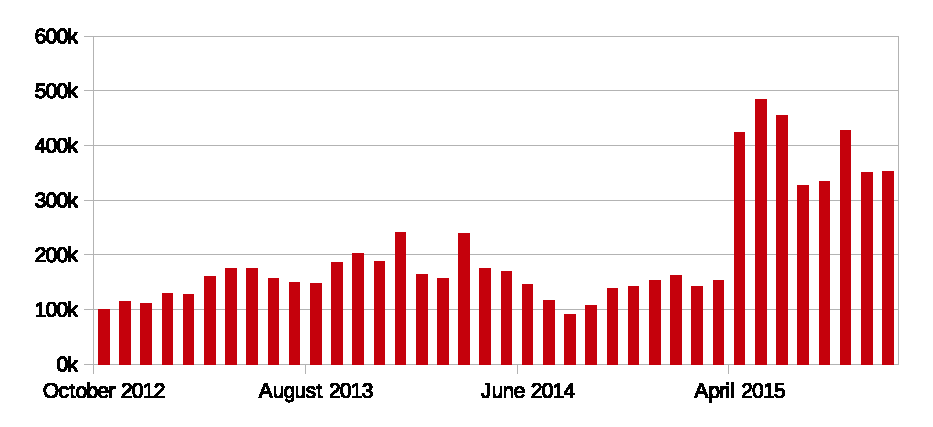
\includegraphics[width=8.6cm]{querylogs}
\caption{Amount of queries on the route planning part of the iRail API between October 2012 and December 2015. In April 2015 an official app of the Belgian railways was discontinued, which explains the sudden raise of iRail API queries.}
\label{fig:querylogs}
\end{figure}

In \cref{fig:querylogs} we show the amount of queries per month.
We can see a sudden grow in April 2015: this is when an official app of the Belgian railway company was discontinued\footnote{\url{https://hello.irail.be/2015/04/22/april-updates/}} and many people started looking for an alternative within the apps built on top of the iRail API.
In 2012, 2013, 2014 and 2015, there were respectively 19.3, 19.4, 19,6 and 19.7 million passengers per month on average\footnote{Calculated by using indicators of the Flemish government and extrapolating the numbers for 2015 \url{http://www4.vlaanderen.be/sites/svr/Cijfers/Exceltabellen/mobiliteit/vervoersprestaties/personenvervoer/MOBIOPEN006.xls}}.
The amount of iRail queries per month, on average in these years are respectively 0.11, 0.17, 0.15 and 0.33 million.
If we assume that each request is a travel intention, this would result in respectively $0.56\%$, 0.88\%, 0.77\% and 1.66\% of the travels that are captured with the iRail API.

\begin{figure}
\centering
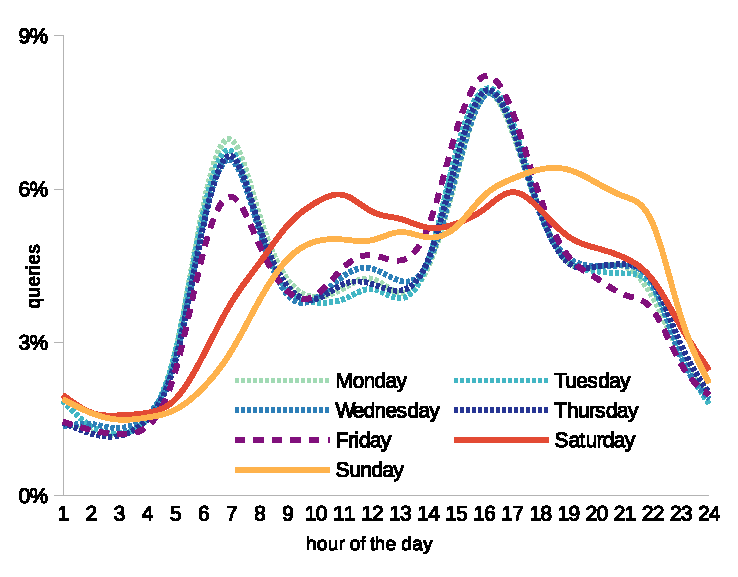
\includegraphics[width=8.6cm]{avg-all}
\caption{Distribution of iRail route planning API queries on average per day of the week between October 2012 and December 2015}
\label{fig:average}
\end{figure}

Next, we made a distribution of the requests done on each day of the week, which resulted in \cref{fig:average}.
In this chart we can spot, on Monday until Friday, the morning peak between 5 and 9 and the evening peak between 15 and 18.
We see a small dent during noon \todo{any explanation for this?}.
On Fridays we see that the morning peak is stronger than the morning peak, which can be explained by many students that go home to visit their parents for the weekend \todo{Can we give a link to more reading material about this behaviour? This might be weird for US people?}.
On Saturdays, we almost do not see the peaks, which can be explained by people not going to work on weekends.
On Sundays, we see most requests happen in the evening, which can be explained by students returning to college accomodations.

\begin{figure}
\centering
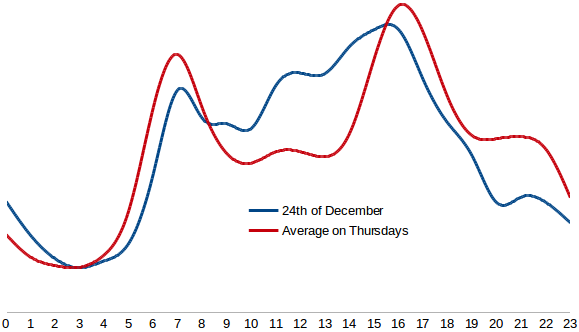
\includegraphics[width=8.6cm]{dec24}
\caption{Comparison of route planning queries on December 24th (Christmass Eve) 2015 with the average on a Thursday between October 2012 and December 2015. The illustration shows that people started going home earlier than usual.}
\label{fig:dec24}
\end{figure}

Finally, we compared the average distribution of Thursdays with the distribution on Thursday the 24th of December 2015 (Christmass Eve).
Our hypothesis that we would now see an earlier evening peak can be confirmed by \cref{fig:dec24}.

We conclude that the timing of the queries look interesting for flow analysis. 
Can we also find interesting patterns when we study where people are heading between certain time intervals?

\section{Method}
\label{sec:method}

Flow analysis involves the comparison of aggregated movement between distinct locations within a specific time frame. 
In most cases, the analytical objective is to identify trends that occur in journeys made  between pairs of locations and allow for their sensitivites to be explored. 
Data visualization is typically employed to facilate in this process thus the input data must be transformed into a format that allows for the quantity and directional flow of movment to be visually encoded. In this section we describe the data transformation procedure and data visualisation technique employed in our case study.

\subsection{Processing}

Matching pairs of origin and destination (OD) stations must be aggregated prior to visualisation.
Several stages of data processing are required to arrive at this outcome.
As we were specifically interested in studying morning and evening rush hour travel that occur on weekdays, we filtered the dataset to exclude data records created outside the time range of 06:00 hrs and 10:00 hrs as well as 17:00 hrs and 21:00 hrs on weekdays, and all data records created on weekend.
\todo{PC: we will have to explain ourselves why we'd choose different hours than what we've found above} 
Queries made by automated user agents like search engine bots and data harvesters were also excluded from the dataset to remove biases that may over represent connections between certain stations. 
Similarly, data records with unparsable origin or destination station names due to invalid character encoding were removed. 
One distinctive challenge is the substantial amount of inconsistency in the way station names are logged. 
Spelling mistakes as well as the use of unstandardized abbreviations in particular, reduce the quality and accuracy of the resulting visualisation.
To overcome this challenge, an open-source reconciliator (https:// github.com/ irail/ stations) was employed to reduce spelling variations and correct identifiable errors. 

The data is then aggregated so that province level flow patterns are emphasised.
\cref{fig:brussels} provides a diagrammatic representation of the procedure.
First, both origin and destination stations for each data record are spatially aggregated based on provincial administrative boundaries (See \cref{fig:brussels}a).
If an origin or destination station is a located outside of Belgium, it is considered international travel and aggregated in a distinct group (See \cref{fig:brussels}b).
Train stations in major cities are excluded from aggregation so that the volume of flow between provinces and major cities are comparable (See \cref{fig:brussels}c).
The following types of flows are observable from the outcome of aggregation:

\begin{itemize}
  \item Travel from any provincial station to a major city.
  \item Travel between any two major cities.
  \item Travel between any two provincial stations.
  \item Travel between any international station to a major city.
  \item Travel between any international station to a provincial station.
\end{itemize}

\subsection{Visualization}

\todo{Alvin} 

\section{Results}
\label{sec:results}

In this chapter, we report on the results of studying visualizations with experts of Trein Tram Bus, a not for profit passenger federation.

\subsection{Commuting pattern}

We see people leaving in the morning and return in the evening (see \cref{fig:brussels} and todo)

The pair of chord diagrams in \cref{fig:brussels,fig:antwerp} capture the aggregated number of queries made between any two stations on weekdays and weekends between 6 to 9 in the morning.
The chords that link two distinct stations, are coloured coded by region and proportionately scaled to the number of queries from a station of origin to a destination.
For instance, approximately 3,530 queries were made from Leuven to Brussels than in the opposite direction (approximately 1,530) on weekdays.
Reading both diagrams in this manner reveals the complexity of movement on the rail system and the significance of cities in daily travel.
Brussels serves as the principal centre of rail activity in general, yet its centrality is more distinctive for the walloon region than Flanders.
Queries from Walloonia with exception to Liege, are generally made from provincial stations towards Brussels instead of their respective provincial capitals.
Queries in Flanders, on the hand, tend to be distributed among major cities otherwise known as the Flemish Diamond, a network of four metropolitan areas in Belgium comprised of Ghent, Brussels, Antwerp and Leuven.
The difference between both patterns appear to correspond with existing measures of population density, providing valuable insight and alternative perspectives into the function of cities in rural and urban settings.

\subsection{Flanders is polycentric, Wallonia monocentric}


\begin{figure}
\centering
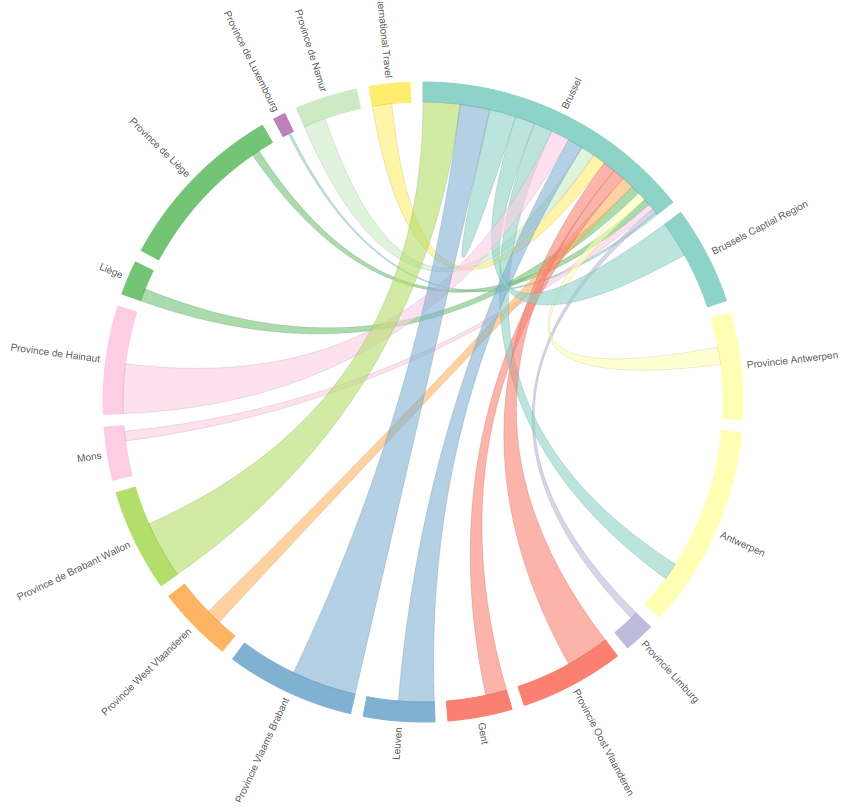
\includegraphics[width=8.1cm]{brussels}
\caption{Pair of chord visualization of the city of Brussels: transit flows towards Brussels from elsewhere in Belgium and vice versa.}
\label{fig:brussels}
\end{figure}

\begin{figure}
\centering
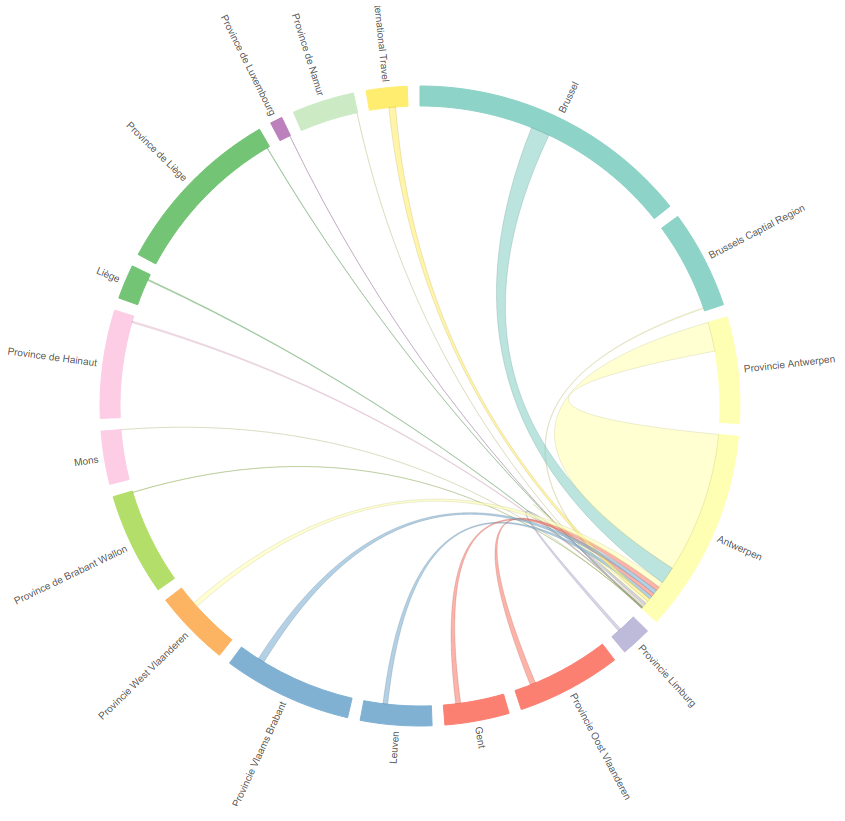
\includegraphics[width=8.1cm]{antwerp}
\caption{Pair of chord visualization of the city of Antwerp: transit flows towards Antwerp from elsewhere in Belgium and vice versa.}
\label{fig:antwerp}
\end{figure}

We can also observe the effect of "density" in Flanders where people move from the rural towards cities. Look at weekday-mornings: commuting towards Gent, Brussels, Antwerp. This is not as obvious in the Walloon region (except for Liege). The reverse occurs on weekday-evenings. Local patterns can also be observed and this corresponds to what we know: ``cities are the central hubs''.
Walloon region: everything converges on Brussels

\subsection{Inexplicable results}

We also see weird things happening in Antwerp, where a large amount of people go to the province in the morning on weekdays, while the oposite happens in Liege.
When looking into the data, the Antwerp pattern appears due to one specific route which is queried each morning.
Is there a group of colleagues all using the same app taking the same train daily?
Is it someone who checks this trip over and over again for delays?
We can only guess\ldots

\section{Publishing transport data}
\label{sec:publishing}

%It is in the interest of public transit agencies that the use of their time schedule data is maximized.
%We can imagine that when more people are informed about the agency's offer, there will be a higher amount of people that will use the service.
%There are currently two ways to publish transit data, as illustrated in \cref{fig:LDFAxis2}: publishing data using the General Transit Feed Specification (GTFS) and offering a route planning service.

%\emph{GTFS}, on the one hand, is a data dump format: it is a compressed ZIP-file, containing a couple of CSV files, describing the rules for when a public transit vehicle will pass by on a certain location.
%GTFS is supported among all current open source route planning software systems and it is used in products/apps such as \emph{CityMapper}, \emph{Ally}, \emph{Navitia.io}, \emph{Google Maps} and \emph{Bing Maps}.
%Persistence of the identifiers used within these datasets, is not a requirement, neither is it an ambition of the format\footnote{\url{https://groups.google.com/forum/#!msg/gtfs-changes/Z8Mf31MaZms/8Hc9F4psAQAJ}}.
%The goal of GTFS is to create an exchange format which specific software packages can use to transform it into their format of choice.

%On the other hand, public transit agencies also publish their data by providing \emph{route planners} such as the French railway company\footnote{\url{http://tech.eu/features/7119/sncf-api-real-time-data/}}, the Dutch railway company\footnote{\url{http://www.ns.nl/reisinformatie/ns-api}} or \ldots\footnote{\url{http://otherapiofadifferentagency}}
%These route planner offer a query service on top of the data and expose these over the Web.
%In this paper we have studied the query logs of such an \emph{expressive} route planning API, which per request offers an interesting log entry.


%label: fig:LDFAxis2

% Linked Data Fragments axis
\begin{figure}[t]
  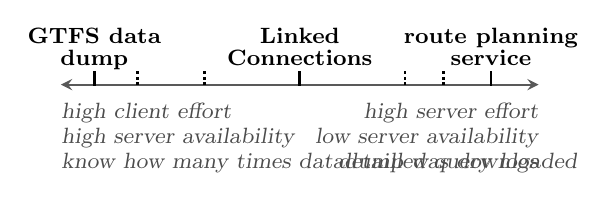
\begin{tikzpicture}[
    x=.005\textwidth,
    y=.1cm,
    axis/.style={
      line width=.8pt,
      stealth-stealth,
      color=black!65,
    },
    axislabel/.style={
      inner sep=0,
      font=\slshape\fontsize{8}{9}\selectfont,
      color=black!70,
    },
    tick/.style={
      line width=1pt,
    },
    ticklabel/.style={
      anchor=south,
      inner sep=0,
      align=center,
      font=\bfseries\fontsize{8}{8}\selectfont,
      text depth=0pt,
    },
  ]
    \newcommand\tick[2]{%
      \draw[tick] (#1, 1.7) -- (#1, -.4pt);
      \node[ticklabel] at (#1, 2.4) {#2};
    }
    \newcommand\vaguetick[1]{%
      \draw[tick,densely dotted] (#1, 1.7) -- (#1, -.4pt);
    }

    \draw[axis] (-100, 0) -- (0, 0);
    \node[axislabel,align=left,anchor=north west] at (-100, -2.3)
    {
%      generic requests\\
      high client effort\\
      high server availability\\
      know how many times datadump was downloaded
    };
    \node[axislabel,align=right,anchor=north east] at (0, -2.3)
    {
%      specific requests\\
      high server effort\\
      low server availability\\
      detailled query logs
    };

    \tick{-93}{GTFS data\\dump}
    \tick{-10}{route planning\\service}
    \tick{-50}{Linked\\Connections}

    \vaguetick{-84}    \vaguetick{-70}
    \vaguetick{-10}
    \vaguetick{-28}
    \vaguetick{-20}

   %\node[align=center,font=\fontsize{8}{9}\selectfont\bfseries] at (0, -8.3)
   %   {various types of\\Linked Data Fragments};
  \end{tikzpicture}
  \caption{This axis extends \cref{fig:LDFAxis1} with Linked Connections: a different choice of trade-offs for route planning advice over the Web.
  }
  \label{fig:LDFAxis2}
\end{figure}

%Linked Data Fragments~\cite{ldf} is a way to think about data publishing as a set of trade-offs between client and servers.
%These trade-offs can be visualized on the axis in \cref{fig:LDFAxis2}: ticks in between the extremes indicate different client/server options.
%For route planning systems, we call these other ticks Linked~Connections~\cite{lc}: 
%by publishing fragments of the data needed by an earliest arrival time algorithm, the algorithm can be executed by a user agent while the downloading the data.
%An example of such an implementation is illustrated in \cref{fig:lc}.
%By exploiting the caching mechanisms behind HTTP, it lowers to load on the server, making it easier to keep the data high available.
%Furthermore, it enables clients to federate queries over different servers representing different regions, transit modes or different user requirements such as low criminality rates or wheelchair accessibility.


%\begin{figure}[h]
%    \centering
%    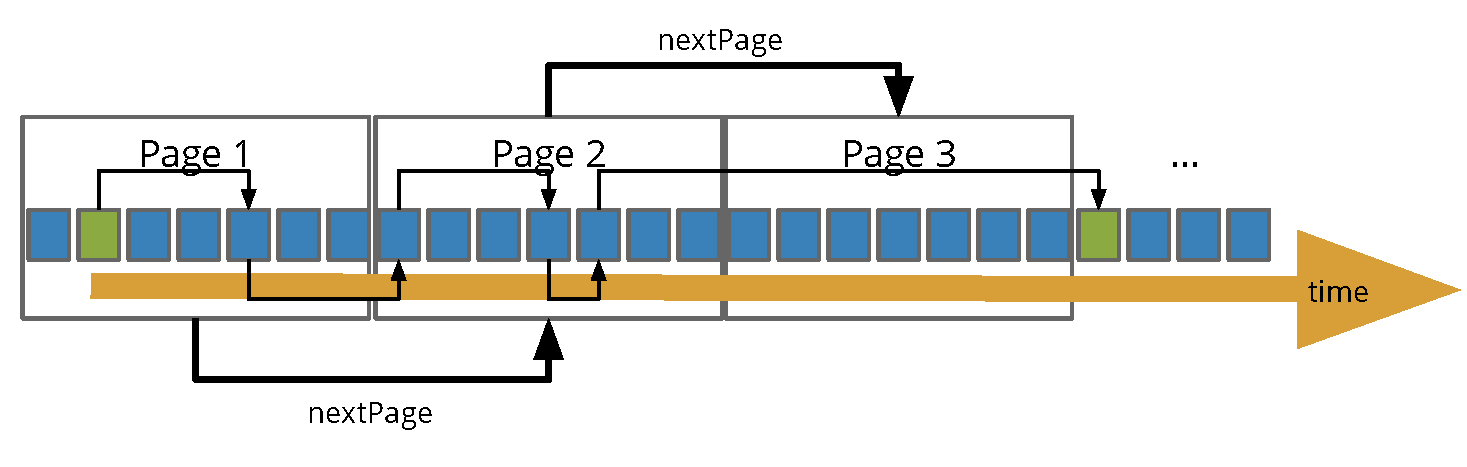
\includegraphics[width=0.48\textwidth]{LC}
%    \caption{An example implementation of a route planning algorithm: fragments of data needed by a route planning algorithm are published in pages. The route planning algorithm will need multiple requests instead of just one. The fragements of the pages that can be retrieved are however highly cacheable.}
%    \label{fig:lc}
%\end{figure}
%

%%% EXPLAIN:
%%%
The expressiveness of a server affects the way logs can be gathered.
We have shown in previous sections that the query logs of a \emph{high expressive server}, such as the iRail API, are interesting: each request contains an entire query which can be interpreted as a travel intention.
The possibility that two requests are exactly the same is low, as there are many URLs which can be requested.
Nevertheless, we cannot fully guarantee that each HTTP GET request to the server will trigger a log entry, due to caching mechanisms on the Web~\cite{fielding}, which might lead to a false representation.

%intermodality, features and availability
Hosting a route planning API as the only way to publish transport data comes with three identified limitations, as the server will need to handle the requests from different use cases with different needs:
\begin{enumerate}
  \item When an application developer would like a \emph{new feature}, such as taking wheelchair accessibility information into account, the feature would have to be implemented on the server of the data publisher
  \item Keeping the server \emph{high available} is costly, as any question can be asked by anyone for any purpose.
  \item Federated querying, which would allow for \emph{intermodal} route planning for route planning APIs, is unexistent up to date.
\end{enumerate}

% GTFS
In order to overcome these limitations, the General Transit Feed Specification (GTFS)\footnote{\url{https://developers.google.com/transit/gtfs/reference}} can be used. 
GTFS is a compressed ZIP-file containing a couple of CSV files, describing the rules for when a public transit vehicle will pass by on a certain location.
It is supported among all current open source route planning software systems and it is used in products/apps such as \emph{CityMapper}, \emph{Ally}, \emph{Navitia.io}, \emph{Google Maps} and \emph{Bing Maps}.
%Persistence of the identifiers used within these datasets, is not a requirement, neither is it an ambition of the format\footnote{\url{https://groups.google.com/forum/#!msg/gtfs-changes/Z8Mf31MaZms/8Hc9F4psAQAJ}}.
%The goal of the format is to  an exchange format which specific software packages can use to transform it into their format of choice.
It succesfully enabled reuse for intermodal travel, engineers can rely on the data dumps even if the servers of the transit agency are offline and there is no limitation to the features that can be implemented.
The logs are however lost.

In \cref{fig:LDFAxis2} we illustrate these two options as two extremes, with other options that are yet to be discovered.
When a \emph{rather low expressive} server only allows to set e.g., a departure station and a departure time, then the server cannot log the arrival station, yet the client is still able to plan a route by executing the algorithm on the client-side~\cite{lc}.
We would be able to fully rely on the query logs if the expressivity would be maximal (extreme right) and caching would be turned off.
Turning off caching may work in a private setting where you know how much and what kind of queries you can expect, yet on the Web, it will not scale up.\todo{PC: Just being devil's advocate here: is caching really necessary to scale sufficiently?}

\section{Publishing query logs}
\label{sec:publishingquerylogs}

IRail is a not for profit organization that stimulates digital creativity concerning mobility.
The interface that takes care of the route planning interface is open source, and we could easily suggest a change to the system in which the query logs become open\footnote{\url{https://github.com/iRail/iRail/pull/138}}.
As of the 17th of December 2015, iRail publishes the most recent 1000 requests done on the API as open data, each second, at \url{http://api.irail.be/logs/}.

In order to publish this data, we chose a newline-based format: each new line contains a new query object encoded in JSON. 
We call this a \emph{JSON-stream}, as the JSON objects can be read one per one.
Unix commands such as \emph{grep} work well with this format.
We chose this over CSV as we have more flexibility towards changing the object properties.


\todo{Also in USEWOD2014 there was a paper on LDF and how we could know which SPARQL queries needed to be solved}

\todo{As of the 17th of December 2015, iRail publishes the most recent 1000 requests done on the API as open data, each second, at \url{http://api.irail.be/logs/}.
This amounts today to an average of 86k queries to the API per day, as the API gained popularity thanks to apps like \emph{BeTrains}\footnote{\url{https://play.google.com/store/apps/details?id=tof.cv.mpp}} and \emph{Railer}\footnote{\url{http://railer.be/}}.
On average, 14,357 of these are valid route planning queries (other queries include requesting departures in a station, status of a vehicle, or a list of all stations).
If each query would amount to indeed one passenger, this would today be equal to almost 2\% of all passengers.}

\section{Conclusion and future work}
\label{sec:conclusion}

The contribution of this paper is twofold.
For the first time, we studied query logs to find travel patterns.
Due to lack of information we could not evaluate our results, yet the visualizations look promising...
There are obvious caveats associated with the use of such data as proxy for actual statistical counts. 
For instance, the data only captures an intention of a passenger: it's unsure whether the person actually took the train.
Furthermore, different requests could be done by one person with an intention to travel.
On top of that, our sample used for this paper can only represent a maximum of 0.4\% of the daily traffic flow.

The second contribution is our position that we suggest to decouple the query logs from the query execution.

In future work, iRail will try to use these to predict train congestion.
% Fix spacing after References header (as line 1308 of sig-alternate.cls breaks it)
\let\oldsection\section
\renewcommand{\section}[2][1]{\oldsection{#1}\vspace{-3pt}}

\bibliographystyle{abbrv}
\bibliography{refs}
\end{document}
